\documentclass[tikz,border=7pt]{standalone}
\usepackage[T1]{fontenc}
\usetikzlibrary{arrows.meta}
\begin{document}
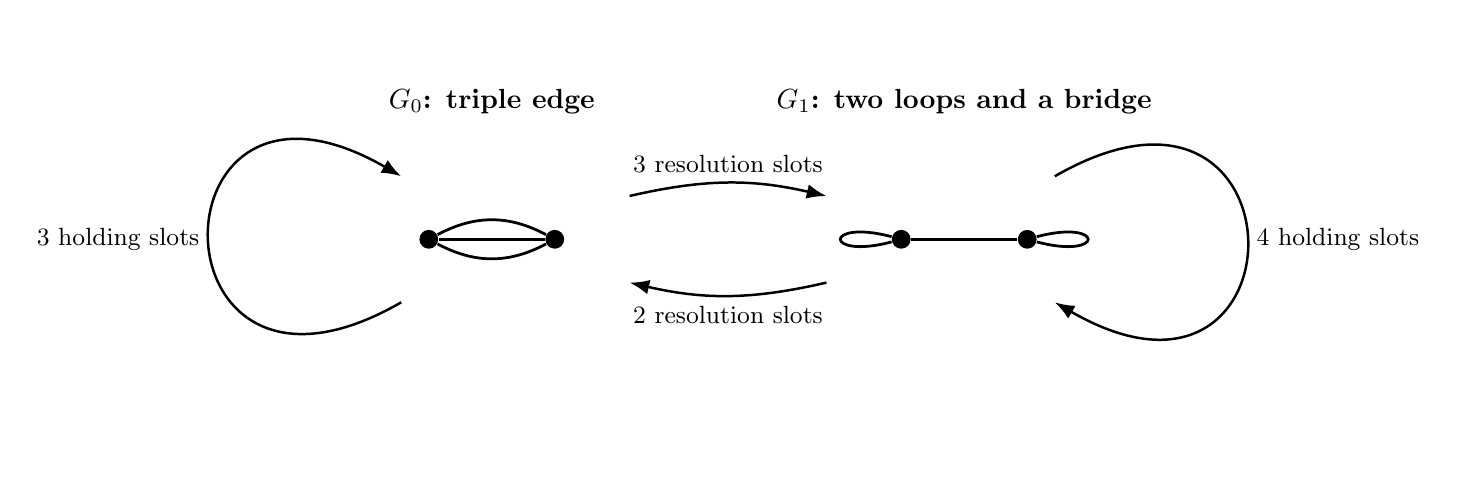
\begin{tikzpicture}[
  vertex/.style={circle,fill=black,inner sep=2.4pt},
  edge/.style={line width=1pt},
  arrow/.style={-{Latex[length=2.5mm]},line width=.9pt},
  every node/.style={font=\small}
]
  \node[font=\bfseries] at (-3,1.75) {$G_0$: triple edge};
  \node[vertex] (a0) at (-3.8,0) {};
  \node[vertex] (b0) at (-2.2,0) {};
  \draw[edge] (a0)--(b0);
  \draw[edge] (a0) to[bend left=28] (b0);
  \draw[edge] (a0) to[bend right=28] (b0);

  \node[font=\bfseries] at (3,1.75) {$G_1$: two loops and a bridge};
  \node[vertex] (a1) at (2.2,0) {};
  \node[vertex] (b1) at (3.8,0) {};
  \draw[edge] (a1)--(b1);
  \draw[edge] (a1) edge[loop left,min distance=9mm] (a1);
  \draw[edge] (b1) edge[loop right,min distance=9mm] (b1);

  \draw[arrow] (-1.25,.55) to[bend left=13]
    node[above] {$3$ resolution slots} (1.25,.55);
  \draw[arrow] (1.25,-.55) to[bend left=13]
    node[below] {$2$ resolution slots} (-1.25,-.55);
  \draw[arrow] (-4.15,-.8) to[out=210,in=150,looseness=6]
    node[left] {$3$ holding slots} (-4.15,.8);
  \draw[arrow] (4.15,.8) to[out=30,in=-30,looseness=6]
    node[right] {$4$ holding slots} (4.15,-.8);
\end{tikzpicture}
\end{document}
